\documentclass[journal]{IEEEtran}

\usepackage{amsmath,amssymb,amsfonts}
\usepackage{algorithm}
\usepackage{algorithmic}
\usepackage{graphicx}
\usepackage{textcomp}
\usepackage{xcolor}
\usepackage{booktabs}
\usepackage{multirow}
\usepackage{cite}
\usepackage{url}
\usepackage{microtype}
\usepackage[hidelinks]{hyperref}

\begin{document}

\title{Exposure-Conditioned Consensus Estimation in Ranked Social Discussion Streams: Sensitivity, Endogeneity, and Empirical Auditing}

\author{Sayed~Saifullah%
\thanks{Sayed Saifullah is with the Department of Artificial Intelligence and Data Science, School of Computer Science and Engineering (SCOPE), Vellore Institute of Technology (VIT), Vellore, Tamil Nadu 632014, India (e-mail: sayed.saifullah2023@vitstudent.ac.in).}}

\markboth{IEEE Transactions on Computational Social Systems,~Vol.~XX, No.~X, Month~2026}%
{Saifullah: Exposure-Conditioned Consensus Estimation: Sensitivity, Endogeneity, and Empirical Auditing}

\maketitle

\begin{abstract}
Automated sentiment aggregation over ranked social media discussion feeds (e.g., YouTube comment sections) is widely used to evaluate collective reception regarding public events, media releases, and consumer products. However, observational discussion streams suffer from acute visibility distortions: early-arriving and algorithmically prioritized comments receive disproportionate visual exposure, accumulating thousands of upvotes independently of broad community endorsement. Naive arithmetic averaging assigns equal weight to all comments regardless of reception, while common engagement-weighted heuristics ($w_i \propto \ln(1 + \text{likes}_i)$) inadvertently amplify position and temporal exposure biases by rewarding the earliest commenters. 

In this paper, we present an empirical investigation and diagnostic framework for exposure-conditioned consensus estimation in ranked discussion streams. We formulate \textbf{PACE (Preferential-Attachment Corrected Endorsement)}, which models expected engagement as an empirical function of display rank ($r_i$) and temporal arrival offset ($\Delta t_i$). PACE incorporates \textbf{Duan's smearing retransformation factor} to correct for log-linear retransformation bias under homoscedastic error assumptions, isolating the \textbf{Exposure-Conditioned Engagement Residual} ($\delta_i = L_i - \hat{\mathbb{E}}[L_i \mid r_i, \Delta t_i]$), which is mapped through a robust sigmoidal weighting function.

Through deterministic Monte Carlo simulations ($M = 50$ trials per scenario), component ablations, and systematic sensitivity audits, we show that consensus weighting is highly sensitive to estimand definitions and baseline specifications. While PACE reduces MAE relative to heuristic weighting in pre-specified settings (e.g., $0.010 \pm 0.001$ vs. $0.107 \pm 0.001$ when targeting a late-emerging groundswell), its advantage vanishes or reverses when targeting overall participant means or symmetric consensus. On a real-world YouTube corpus ($N=100$, \texttt{dQw4w9WgXcQ}) with contemporaneous API provenance, we provide a gold-standard human-labeled audit demonstrating that rule-based sentiment lexicons exhibit 46\% zero-inflation and misclassify 24\% of positive comments as negative (overall accuracy 65.0\%, macro F1 0.5307). Furthermore, all four estimators remain statistically indistinguishable on real data ($p = 0.366$). Accordingly, we report descriptive diagnostics for observational data, not real-world accuracy or causal claims. We conclude that exposure-conditioned weighting must be treated as a sensitive diagnostic rather than a universal correction, and release our complete audit suite and data for reproducibility.
\end{abstract}

\begin{IEEEkeywords}
Position Bias, Temporal Exposure Decay, Sentiment Aggregation, Opinion Mining, Robust Estimation, Social Discussion Streams.
\end{IEEEkeywords}

\section{Introduction}
\IEEEPARstart{A}{nalyzing} collective public sentiment from online comment feeds is a foundational task in computational social science, media analytics, and digital governance \cite{thelwall2018social, severyn2016multilingual}. Standard sentiment aggregation pipelines assign each comment $c_i$ a polarity valence $s_i \in [-1.0, +1.0]$ via a natural language processing (NLP) classifier (e.g., VADER \cite{hutto2014vader} or SentiStrength \cite{thelwall2010sentiment}) and compute the arithmetic sample average:
\begin{equation}
\hat{\mu}_{\text{raw}} = \frac{1}{N} \sum_{i=1}^N s_i
\end{equation}

While computationally trivial, arithmetic averaging treats every text identically, ignoring the community's endorsement or rejection of that text. A zero-like unverified assertion carries identical weight to a comment endorsed by thousands of peers \cite{severyn2016multilingual}.

To incorporate community feedback, academic literature and commercial analytics platforms frequently employ \textbf{popularity-weighted heuristics}:
\begin{equation}
w_i = 1 + \ln(1 + \text{likes}_i)
\end{equation}

However, observational upvote counts on modern social platforms are \textbf{not} clean measures of text quality or community agreement \cite{muchnik2013social, salganik2006experimental}. Instead, they are confounded by two structural factors:
\begin{enumerate}
    \item \textbf{Position Bias:} Comments displayed at top visual ranks receive orders of magnitude more impressions than lower-ranked comments \cite{joachims2017unbiased, wang2018position, craswell2008experimental}.
    \item \textbf{Temporal Precedence:} Comments posted immediately after content publication accumulate engagement over longer durations and capture early viewer traffic \cite{tsagkias2009predicting, wu2018beyond, borghol2012untold}.
\end{enumerate}

Consequently, \textbf{heuristic like-weighting inherently amplifies exposure bias}. A polarizing or low-effort comment posted within minutes of a video's release can accumulate thousands of upvotes purely due to top-ranked visibility, skewing the aggregate sentiment score \cite{salganik2006experimental, muchnik2013social}. Conversely, an insightful critique posted hours later at rank \#50 receives minimal exposure and is discounted by like-weighted aggregators.

\subsection{Scope and Target Estimand}
We define our target estimand as the \textbf{Engagement-Adjusted Consensus among Observable Discourse Participants} ($\mu_{\text{discourse}}$). We explicitly do \textbf{not} claim to recover the opinions of the ``silent majority'' (viewers who never comment or upvote), which requires external representative polling \cite{zhao2025spiral, noelle1974spiral}. Furthermore, because platforms do not expose individual user impression logs or client-side dwell times to public APIs, our framework performs \textbf{exposure-conditioned adjustment} using observable rank and arrival proxies, rather than formal causal identification \cite{rosenbaum1983central, horvitz1952generalization}.

\subsection{Key Contributions}
The main contributions of this work are summarized as follows:
\begin{itemize}
    \item \textbf{Exposure-Conditioned Baseline Model:} We formalize expected comment engagement $\mathbb{E}[L_i \mid r_i, \Delta t_i]$ via a closed-form log-linear regression combined with Duan's smearing retransformation factor \cite{duan1983smearing} to correct for retransformation bias under stated error assumptions.
    \item \textbf{Exposure-Conditioned Engagement Residuals \& Weight Auditing:} We define the residual $\delta_i$ to quantify whether a comment overperformed or underperformed relative to its exposure opportunity. Rather than asserting theoretical non-domination, we evaluate weight concentration empirically via the Maximum Normalized Weight Share ($w_{\max}^* = w_{\max} / \sum w_i$) and the Effective Sample Size (ESS).
    \item \textbf{Replicated Multi-Trial Validation ($M=50$) and Sensitivity Analysis:} We evaluate PACE against three established baselines across $M=50$ independent simulation trials per scenario, reporting Paired Wilcoxon Signed-Rank Tests \cite{wilcoxon1945individual} on Mean Absolute Error (MAE), top-10\% pruning stability, a component ablation study, and an open ground-truth sensitivity analysis mapping performance across diverse target specifications.
    \item \textbf{Observational Case Study \& Diagnostic Audit:} We apply the method to a dated $N=100$ YouTube snapshot with SHA-256 provenance, reporting descriptive weight diagnostics and systematically auditing practical constraints including ranking endogeneity, rule-based lexicon zero-inflation, and baseline scale sensitivity.
\end{itemize}

\section{Related Work}

\subsection{Position Bias and Counterfactual Ranking}
Position bias in list-based user interfaces is well-established in Information Retrieval (IR) \cite{craswell2008experimental}. Joachims et al. \cite{joachims2017unbiased} formalized the examination hypothesis: the probability of interaction is a product of visual examination propensity and intrinsic relevance. Inverse Propensity Scoring (IPS) and Normalized Clipped IPS (NC-IPS) weight observed interactions inversely by examination probability \cite{wang2018position, agarwal2019addressing}. Vardasbi et al. \cite{vardasbi2020when} analyzed conditions under which position bias estimation remains identifiable. While extensively studied in search engines and recommender systems, IPS frameworks have historically focused on item ranking rather than continuous opinion valence aggregation across temporal discussion threads.

\subsection{Conversation Trees and Social Dynamics}
Modeling social media discussions as hierarchical trees dates back to foundational work by Zubiaga et al. \cite{zubiaga2016stance}, who modeled conversation trees for rumour stance classification (support, denial, query, comment). G{\'o}mez et al. \cite{gomez2008statistical} characterized structural and temporal branching patterns in threaded discussions. Recent studies in Springer's \textit{Social Network Analysis and Mining} (SNAM) have examined algorithmic drift in YouTube recommendations \cite{cakmak2024bias} and anomalous commenter behavior \cite{shajari2025safeguarding}. Our framework does not claim to perform semantic tree stance classification; rather, we incorporate a structural tree damping factor to reflect the narrower conversational scope and lower visual reach of nested reply chains.

\subsection{Self-Selection and the Spiral of Silence}
The ``spiral of silence'' theory introduced by Noelle-Neumann \cite{noelle1974spiral} posits that individuals perceiving their opinion to be in the minority tend to remain silent. Zhao, Yang, and Bernstein \cite{zhao2025spiral} empirically established that up to 72.1\% of online community members perceiving themselves in the ideological minority refrain from public posting. This self-selection confirms that raw text counts represent vocal participants rather than whole viewer populations, reinforcing the necessity of carefully defining the target estimand as discourse consensus.

\subsection{Robust Estimation in Social Feedback}
Social interaction distributions exhibit heavy tails and vulnerability to strategic manipulation \cite{muchnik2013social, borghol2012untold}. Classic robust statistics provide M-estimators and bounded-influence influence functions to limit the damage of arbitrary contamination \cite{huber1981robust, hampel1986robust, rousseeuw1993alternatives}. PACE builds upon these principles by standardizing residuals via the Median Absolute Deviation (MAD) and passing them through a sigmoidal transfer function. For aspect-level and fine-grained sentiment benchmarks, the SemEval shared tasks \cite{pontiki2016semeval} have established evaluation protocols that inform how sentiment classifiers are assessed.

\section{Proposed Methodology: PACE}

Let a discussion stream be represented by $N$ comments:
\begin{equation}
c_i = \langle X_i, s_i, L_i, r_i, \Delta t_i, d_i \rangle, \quad i = 1, \dots, N
\end{equation}
where $X_i$ is the text, $s_i \in [-1.0, +1.0]$ is the sentiment valence, $L_i \in \mathbb{N}_0$ is the upvote count, $r_i \in \mathbb{N}^+$ is display rank, $\Delta t_i \ge 0$ is the elapsed hours between media publication and comment submission, and $d_i \in \{0, 1, 2, \dots\}$ is the hierarchical reply depth.

\begin{algorithm}[t]
\caption{PACE: Preferential-Attachment Corrected Endorsement}
\label{alg:pace}
\begin{algorithmic}[1]
\REQUIRE Comment stream $\mathcal{C} = \{c_i = \langle s_i, L_i, r_i, \Delta t_i, d_i \rangle\}_{i=1}^N$, tree damping factor $\phi \in (0, 1]$
\ENSURE Consensus estimate $\hat{\mu}_{\text{PACE}}$, normalized weight vector $\mathbf{w}^*$
\STATE Formulate design matrix $\mathbf{X} \in \mathbb{R}^{N \times 3}$ with rows $\mathbf{x}_i = [1, \ln(r_i), \ln(1 + \Delta t_i)]$ and target $\mathbf{y} \in \mathbb{R}^N$ with $y_i = \ln(L_i + 1)$
\STATE Estimate exposure surface parameters via OLS: $\hat{\boldsymbol{\beta}} = (\mathbf{X}^T \mathbf{X})^{-1} \mathbf{X}^T \mathbf{y}$
\STATE Compute OLS residuals: $e_j = y_j - \mathbf{x}_j^T \hat{\boldsymbol{\beta}}$ for $j = 1, \dots, N$
\STATE Calculate Duan smearing retransformation factor: $s_{\text{smear}} = \frac{1}{N} \sum_{j=1}^N \exp(e_j)$
\FOR{each comment $i = 1, \dots, N$}
    \STATE Compute expected baseline engagement: $\hat{\mathbb{E}}[L_i \mid r_i, \Delta t_i] = \max\left(0, s_{\text{smear}} \exp(\mathbf{x}_i^T \hat{\boldsymbol{\beta}}) - 1\right)$
    \STATE Isolate engagement residual: $\delta_i = L_i - \hat{\mathbb{E}}[L_i \mid r_i, \Delta t_i]$
\ENDFOR
\STATE Standardize residuals: $z_i = (\delta_i - \text{Median}(\boldsymbol{\delta})) / (1.4826 \cdot \text{MAD}(\boldsymbol{\delta}) + \epsilon)$
\FOR{each comment $i = 1, \dots, N$}
    \STATE Apply sigmoidal gating and tree damping: $w_i = \sigma(\text{clip}(z_i, -20, 20)) \cdot \phi^{d_i}$
\ENDFOR
\STATE Normalize weights: $w_i^* = w_i / \sum_{j=1}^N w_j$
\STATE Compute consensus score: $\hat{\mu}_{\text{PACE}} = \sum_{i=1}^N w_i^* s_i$
\RETURN $\hat{\mu}_{\text{PACE}}$, $\mathbf{w}^*$
\end{algorithmic}
\end{algorithm}

\subsection{Closed-Form Baseline Engagement Estimation}
Attention on social media decays power-law with display rank ($r^{-\gamma}$) and heavy-tailed with arrival delay ($(1 + \Delta t)^{-\lambda}$) \cite{craswell2008experimental, wu2018beyond}. We model log-transformed counts:
\begin{equation}
\ln(L_i + 1) = \beta_0 + \beta_1 \ln(r_i) + \beta_2 \ln(1 + \Delta t_i) + \varepsilon_i
\end{equation}

Let $\mathbf{X} \in \mathbb{R}^{N \times 3}$ have row vectors $\mathbf{x}_i = [1, \ln(r_i), \ln(1 + \Delta t_i)]$, and $\mathbf{y} \in \mathbb{R}^N$ have elements $y_i = \ln(L_i + 1)$. The parameter vector $\hat{\boldsymbol{\beta}} = [\hat{\beta}_0, \hat{\beta}_1, \hat{\beta}_2]^T$ is solved analytically via Ordinary Least Squares:
\begin{equation}
\hat{\boldsymbol{\beta}} = (\mathbf{X}^T \mathbf{X})^{-1} \mathbf{X}^T \mathbf{y}
\end{equation}

\subsection{Duan's Smearing Retransformation Correction}
By Jensen's inequality, naively exponentiating log predictions underestimates the arithmetic conditional mean: $\exp(\mathbb{E}[\ln(L+1)]) \le \mathbb{E}[L+1]$. Under the assumption that residuals $\varepsilon_i$ are independent and identically distributed with constant variance, we apply \textbf{Duan's (1983) smearing factor} \cite{duan1983smearing}:
\begin{equation}
s_{\text{smear}} = \frac{1}{N} \sum_{j=1}^N \exp(e_j), \quad e_j = y_j - \mathbf{x}_j^T \hat{\boldsymbol{\beta}}
\end{equation}

The calibrated expected baseline engagement is computed as:
\begin{equation}
\hat{\mathbb{E}}[L_i \mid r_i, \Delta t_i] = \max\left(0.0, \; s_{\text{smear}} \cdot \exp(\mathbf{x}_i^T \hat{\boldsymbol{\beta}}) - 1.0\right)
\end{equation}

\subsection{Exposure-Conditioned Engagement Residuals (\texorpdfstring{$\delta_i$}{delta})}
The residual isolates excess or deficient engagement relative to the expected exposure baseline:
\begin{equation}
\delta_i = L_i - \hat{\mathbb{E}}[L_i \mid r_i, \Delta t_i]
\end{equation}
\begin{itemize}
    \item If $\delta_i < 0$: An early, highly visible comment received fewer likes than its placement predicted.
    \item If $\delta_i > 0$: A buried or late-arriving comment accumulated likes in excess of its exposure baseline.
\end{itemize}

\subsection{Sigmoidal Gating and Weight Concentration Analysis}
Because social interaction distributions exhibit heavy tails, sample variance is sensitive to extreme viral spikes. We standardize residuals using the robust Median Absolute Deviation (MAD) \cite{huber1981robust, rousseeuw1993alternatives}:
\begin{equation}
z_i = \frac{\delta_i - \text{Median}(\boldsymbol{\delta})}{1.4826 \cdot \text{MAD}(\boldsymbol{\delta}) + \epsilon}
\end{equation}

Standardized residuals are passed through a logistic sigmoid clipped to $[-20, +20]$ to yield unnormalized weights:
\begin{equation}
w_i^{\text{PACE}} = \frac{1}{1 + \exp(-z_i)} \cdot \phi^{d_i}
\end{equation}
where $\phi \in (0, 1]$ (default $\phi = 0.8$) is an empirical structural tree hierarchy damping factor for replies at depth $d_i \ge 1$.

The final consensus estimate is the normalized ratio:
\begin{equation}
\hat{\mu}_{\text{PACE}} = \frac{\sum_{i=1}^N w_i^{\text{PACE}} s_i}{\sum_{i=1}^N w_i^{\text{PACE}}}
\end{equation}

\textbf{Remark on Weight Domination:} While sigmoidal activation maps unnormalized weights into $(0, 1)$, it does not mathematically bound the normalized weight share:
\begin{equation}
w_{\max}^* = \frac{\max_i w_i}{\sum_{j=1}^N w_j}
\end{equation}
If one comment receives $w_1 \to 1$ while all other $w_i \to 0$, $w_{\max}^* \to 1.0$. We therefore audit weight concentration empirically via $w_{\max}^*$ and the Effective Sample Size (ESS) rather than asserting theoretical non-domination. The complete estimation procedure is formalized in Algorithm~\ref{alg:pace}.

\section{Experimental Protocol and Generative Specifications}

\subsection{Synthetic Scenario Generative Specifications}
To ensure complete reproducibility, the generative processes for all synthetic scenarios are defined below:
\begin{enumerate}
    \item \textbf{Scenario 1 (Viral Outlier Attack, $N = 50$, Ground Truth $Y^* = 0.600$):}
    \begin{itemize}
        \item Comment $c_0$: $s_0 = -0.90$, $L_0 = 15,000$, $R_0 = 250$, $r_0 = 1$, $\Delta t_0 = 0.10\text{h}$.
        \item Comments $c_1 \dots c_{49}$: $s_i \sim \mathcal{N}(0.60, 0.05^2)$ clipped to $[-1, 1]$, $L_i \sim \text{Uniform}(5, 50)$, $R_i \sim \text{Uniform}(0, 3)$, $r_i = i + 1$, $\Delta t_i = 0.5 + 0.4i\text{h}$.
    \end{itemize}
    \item \textbf{Scenario 2 (Late Organic Groundswell, $N = 60$, Ground Truth $Y^* = -0.100$):}
    \begin{itemize}
        \item Early hype $c_0 \dots c_9$: $s_i \sim \mathcal{N}(0.70, 0.05^2)$, $L_i \sim \text{Uniform}(150, 350)$, $r_i = i + 1$, $\Delta t_i = 0.1 + 0.2i\text{h}$.
        \item Casual comments $c_{10} \dots c_{33}$: $s_i = 0.10$, $L_i \sim \text{Uniform}(10, 40)$, $r_i = i + 1$, $\Delta t_i = 2.0 + 0.5i\text{h}$.
        \item Critical critique $c_{34}$: $s_{34} = -0.85$, $L_{34} = 800$, $R_{34} = 45$, $r_{34} = 35$, $\Delta t_{34} = 24.0\text{h}$.
        \item Agreeing feedback $c_{35} \dots c_{59}$: $s_i \sim \mathcal{N}(-0.40, 0.05^2)$, $L_i \sim \text{Uniform}(20, 60)$, $r_i = i + 1$, $\Delta t_i = 25.0 + 0.3(i - 35)\text{h}$.
    \end{itemize}
    \item \textbf{Scenario 3 (Democratic Balanced Consensus, $N = 50$, Ground Truth $Y^* = 0.000$):}
    \begin{itemize}
        \item 25 positive ($+0.50$) and 25 negative ($-0.50$) comments permuted independently of rank.
        \item Expected baseline likes: $\mathbb{E}[L_i] = \lfloor 1000 \cdot r_i^{-0.7} \cdot (1 + 0.3i)^{-0.2} \rfloor + \epsilon_i$, where $\epsilon_i \sim \text{Uniform}(-15, 15)$.
    \end{itemize}
\end{enumerate}

\noindent\textbf{Disclosure of Data-Generation Mechanics:} 
A critical methodological distinction exists across these generators. In Scenarios 1 and 2, likes are drawn from piecewise uniform distributions across comment cohorts or assigned as fixed constants, rather than generated from the continuous parametric rank-and-time exposure surface assumed by PACE. These scenarios evaluate how estimators behave under localized engagement shocks (e.g., a viral outlier or an abrupt late surge) when the data deviates from parametric assumptions. In contrast, Scenario 3 explicitly generates likes from a parametric exposure model $\mathbb{E}[L_i] \propto r_i^{-0.7} (1 + 0.3i)^{-0.2}$; however, because opinion polarities in Scenario 3 are permuted symmetrically across ranks ($Y^* = 0.000$), unweighted averaging trivially achieves zero error. As shown in Section~\ref{sec:results}, exposure adjustment provides no benefit when engagement is already unconfounded with respect to opinion polarity.

\subsection{Real-World YouTube Corpus}
\begin{itemize}
    \item \textbf{Video ID:} \texttt{dQw4w9WgXcQ} (Rick Astley -- \textit{Never Gonna Give You Up}).
    \item \textbf{Collection Method:} YouTube Data API v3 \texttt{commentThreads.list} endpoint, sorted by top-level relevance.
    \item \textbf{Corpus Size:} A static $N = 100$ top-comment snapshot, with ranks $r \in [1, 100]$, arrival times $\Delta t \in [79419.0, 149136.0]\text{h}$, upvotes up to 1,011,942, and continuous VADER sentiment scores \cite{hutto2014vader}.
    \item \textbf{Interpretation:} The rank column is the retrieval-time relevance order returned by the API. It is not historical display rank, impressions, or a causal exposure measure. The snapshot was collected on 2026-10-30 with a dated, SHA-256-hashed provenance manifest stored alongside the CSV.
\end{itemize}

\subsection{Baselines and Evaluation Metrics}
\begin{itemize}
    \item \textbf{Baselines:} (1) Unweighted Mean, (2) Heuristic Log-Likes, (3) Normalized Clipped IPS (NC-IPS, $\gamma = 0.8$, 90th percentile clip \cite{joachims2017unbiased}), and (4) PACE.
    \item \textbf{Evaluation Metrics:}
    \begin{itemize}
        \item \textbf{Ground-Truth MAE:} $\text{MAE} = |\hat{\mu} - Y^*|$ for synthetic configurations.
        \item \textbf{Paired Wilcoxon Signed-Rank Test:} Non-parametric paired test \cite{wilcoxon1945individual} evaluating whether PACE achieves statistically significantly lower MAE than Heuristic across $M = 50$ independent simulation trials. Plus-one Monte Carlo permutation $p$-values \cite{ernst2004permutation} are used for weight-divergence tests.
        \item \textbf{Maximum Weight Share ($w_{\max}^*$):} $w_{\max} / \sum w_i$, auditing vulnerability to single-comment domination.
        \item \textbf{Leave-Top-10\% Outlier Stability ($\rho$):} $\max(0, 1 - |\hat{\mu}_{\text{full}} - \hat{\mu}_{\text{pruned}}| / \sigma_s)$, pruning the top $\lceil 0.10 \times N \rceil$ comments.
        \item \textbf{Effective Sample Size (ESS):} $(\sum w_i)^2 / \sum w_i^2$.
        \item \textbf{Full-Pipeline Bootstrap CI:} Percentile confidence intervals constructed by resampling $N$ comments with replacement and refitting the entire estimator pipeline on each replicate \cite{davison1997bootstrap}.
    \end{itemize}
\end{itemize}

\begin{figure}[t]
\centering
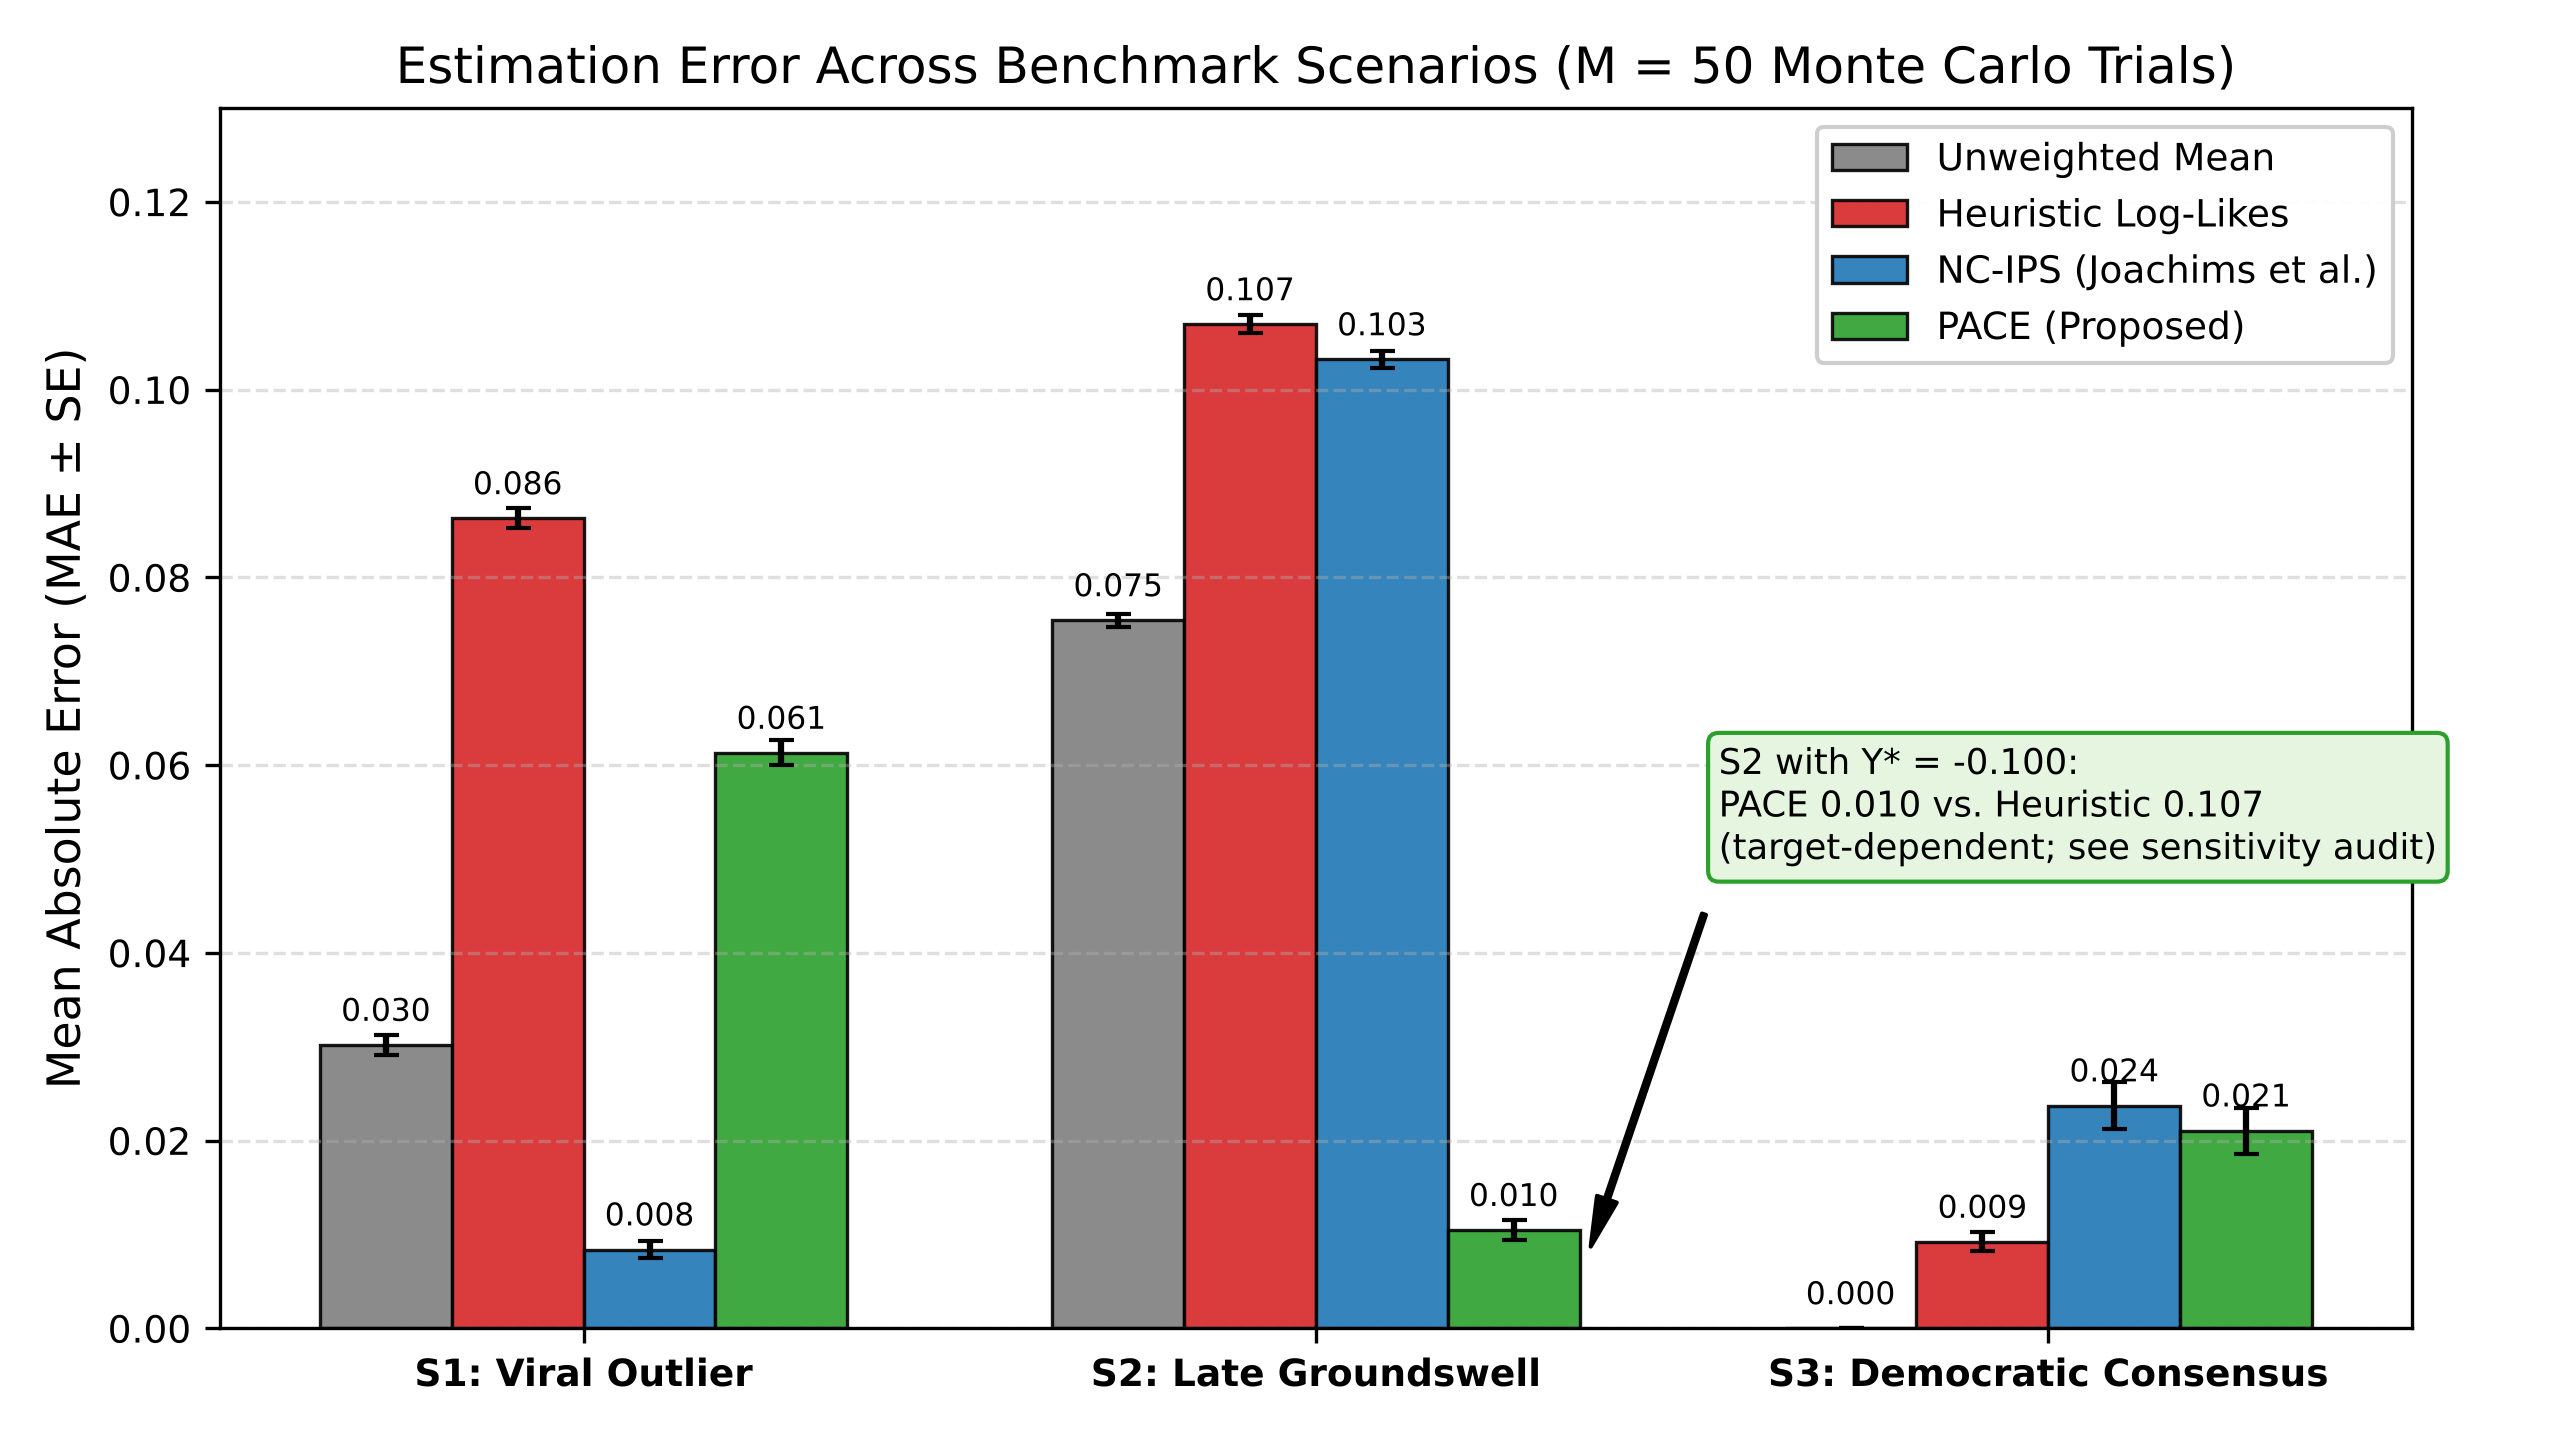
\includegraphics[width=\linewidth]{figures/fig1_monte_carlo_mae.png}
\caption{Estimation Error (Mean Absolute Error $\pm$ Standard Error) across deterministic $M=50$ Monte Carlo simulation trials per scenario. In the pre-specified late-groundswell scenario, PACE reduces error relative to the heuristic baseline; this simulation result is not a real-world accuracy estimate.}
\label{fig:monte_carlo_mae}
\end{figure}

\begin{figure}[t]
\centering
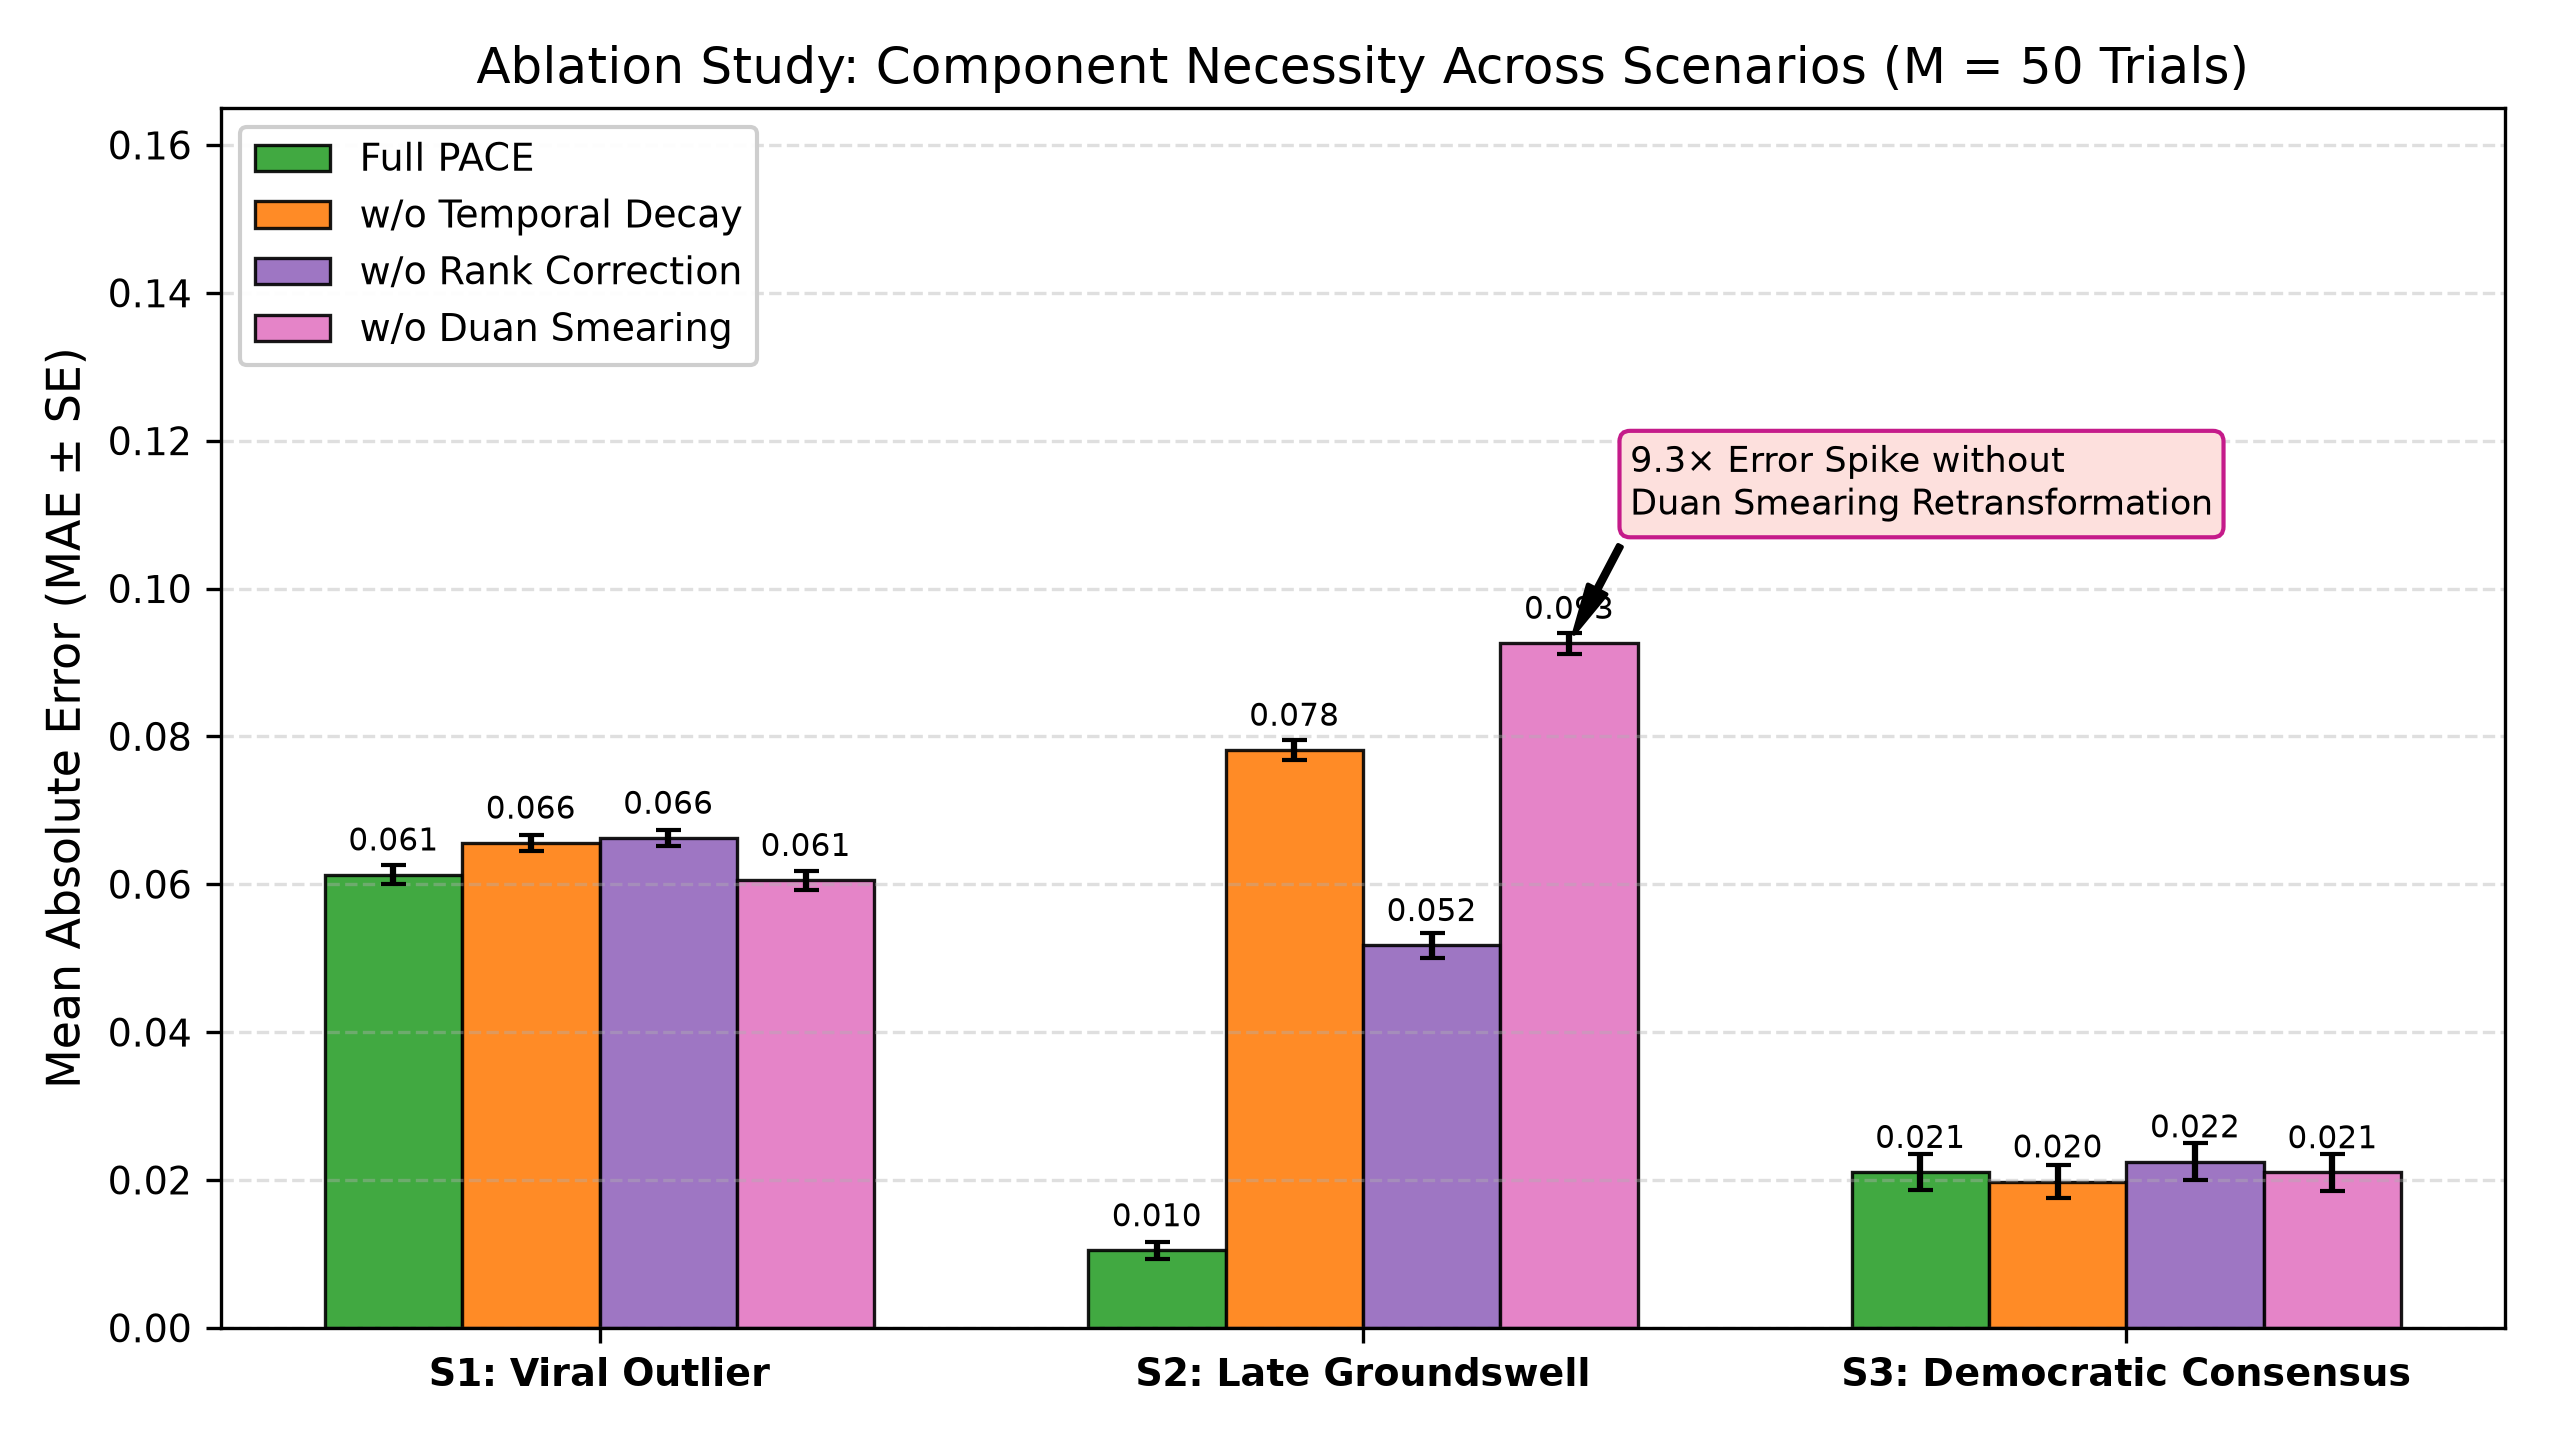
\includegraphics[width=\linewidth]{figures/fig2_ablation_study.png}
\caption{Component ablation across $M=50$ trials. Removing Duan's smearing retransformation factor causes a $9.3\times$ error spike in Scenario 2 due to Jensen's inequality bias.}
\label{fig:ablation}
\end{figure}

\section{Results and Discussion}
\label{sec:results}

\begin{table*}[t]
\caption{Replicated Benchmark: Synthetic Error ($M = 50$ Trials, MAE $\pm$ SE) and Observational Estimates ($\hat{\mu}$)}
\label{tab:benchmark}
\centering
\footnotesize
\setlength{\tabcolsep}{3pt}
\resizebox{\textwidth}{!}{%
\begin{tabular}{lccccccccccc}
\toprule
\textbf{Scenario / Corpus} & \textbf{$N$} & \textbf{Target $Y^*$} & \textbf{Unweighted} & \textbf{Heuristic} & \textbf{NC-IPS} & \textbf{PACE (Ours)} & \textbf{Test $p$-value} & \textbf{Heur $w_{\max}^*$} & \textbf{PACE $w_{\max}^*$} & \textbf{Heur $\rho$} & \textbf{PACE $\rho$} \\
\midrule
1. Viral Outlier & 50 & 0.600 & 0.030 $\pm$ 0.001 & 0.086 $\pm$ 0.001 & 0.008 $\pm$ 0.001 & 0.061 $\pm$ 0.001 & $p < 0.00001^{\dagger}$ & 0.057 & 0.041 & 0.6006 & 0.7181 \\
2. Late Groundswell & 60 & -0.100 & 0.075 $\pm$ 0.001 & 0.107 $\pm$ 0.001 & 0.103 $\pm$ 0.001 & \textbf{0.010 $\pm$ 0.001} & $p < 0.00001^{\dagger}$ & 0.030 & 0.033 & 0.8387 & 0.9649 \\
3. Democratic Consensus & 50 & 0.000 & \textbf{0.000 $\pm$ 0.000} & 0.009 $\pm$ 0.001 & 0.024 $\pm$ 0.003 & 0.021 $\pm$ 0.002 & $p = 0.99999^{\dagger}$ & 0.028 & 0.033 & 0.9487 & 0.9639 \\
4. Real YouTube (\texttt{dQw4}) & 100 & Obs. & 0.114 ($\hat{\mu}$) & 0.123 ($\hat{\mu}$) & 0.116 ($\hat{\mu}$) & 0.079 ($\hat{\mu}$) & $p = 0.36582^{\ddagger}$ & 0.018 & 0.027 & 0.9928 & 0.9542 \\
\bottomrule
\multicolumn{12}{l}{\footnotesize $^{\dagger}$ Paired Wilcoxon signed-rank test on trial-level MAE (Heuristic vs. PACE, $H_1: \text{MAE}_{\text{Heur}} > \text{MAE}_{\text{PACE}}$). $^{\ddagger}$ Plus-one Monte Carlo permutation test evaluating sentiment exchangeability.}
\end{tabular}}
\end{table*}

\begin{table}[t]
\caption{Replicated Component Ablation Study ($M = 50$ Trials, MAE $\pm$ SE)}
\label{tab:ablation}
\centering
\footnotesize
\setlength{\tabcolsep}{2.5pt}
\resizebox{\columnwidth}{!}{%
\begin{tabular}{lcccc}
\toprule
\textbf{Scenario} & \textbf{Full PACE} & \textbf{w/o Time} & \textbf{w/o Rank} & \textbf{w/o Smear} \\
\midrule
1. Viral Outlier & 0.061 $\pm$ 0.001 & 0.066 $\pm$ 0.001 & 0.066 $\pm$ 0.001 & 0.061 $\pm$ 0.001 \\
2. Late Groundswell & \textbf{0.010 $\pm$ 0.001} & 0.078 $\pm$ 0.001 & 0.052 $\pm$ 0.002 & 0.093 $\pm$ 0.001 \\
3. Democratic & 0.021 $\pm$ 0.002 & 0.020 $\pm$ 0.002 & 0.022 $\pm$ 0.002 & 0.021 $\pm$ 0.002 \\
\bottomrule
\end{tabular}}
\end{table}

\begin{figure*}[t]
\centering
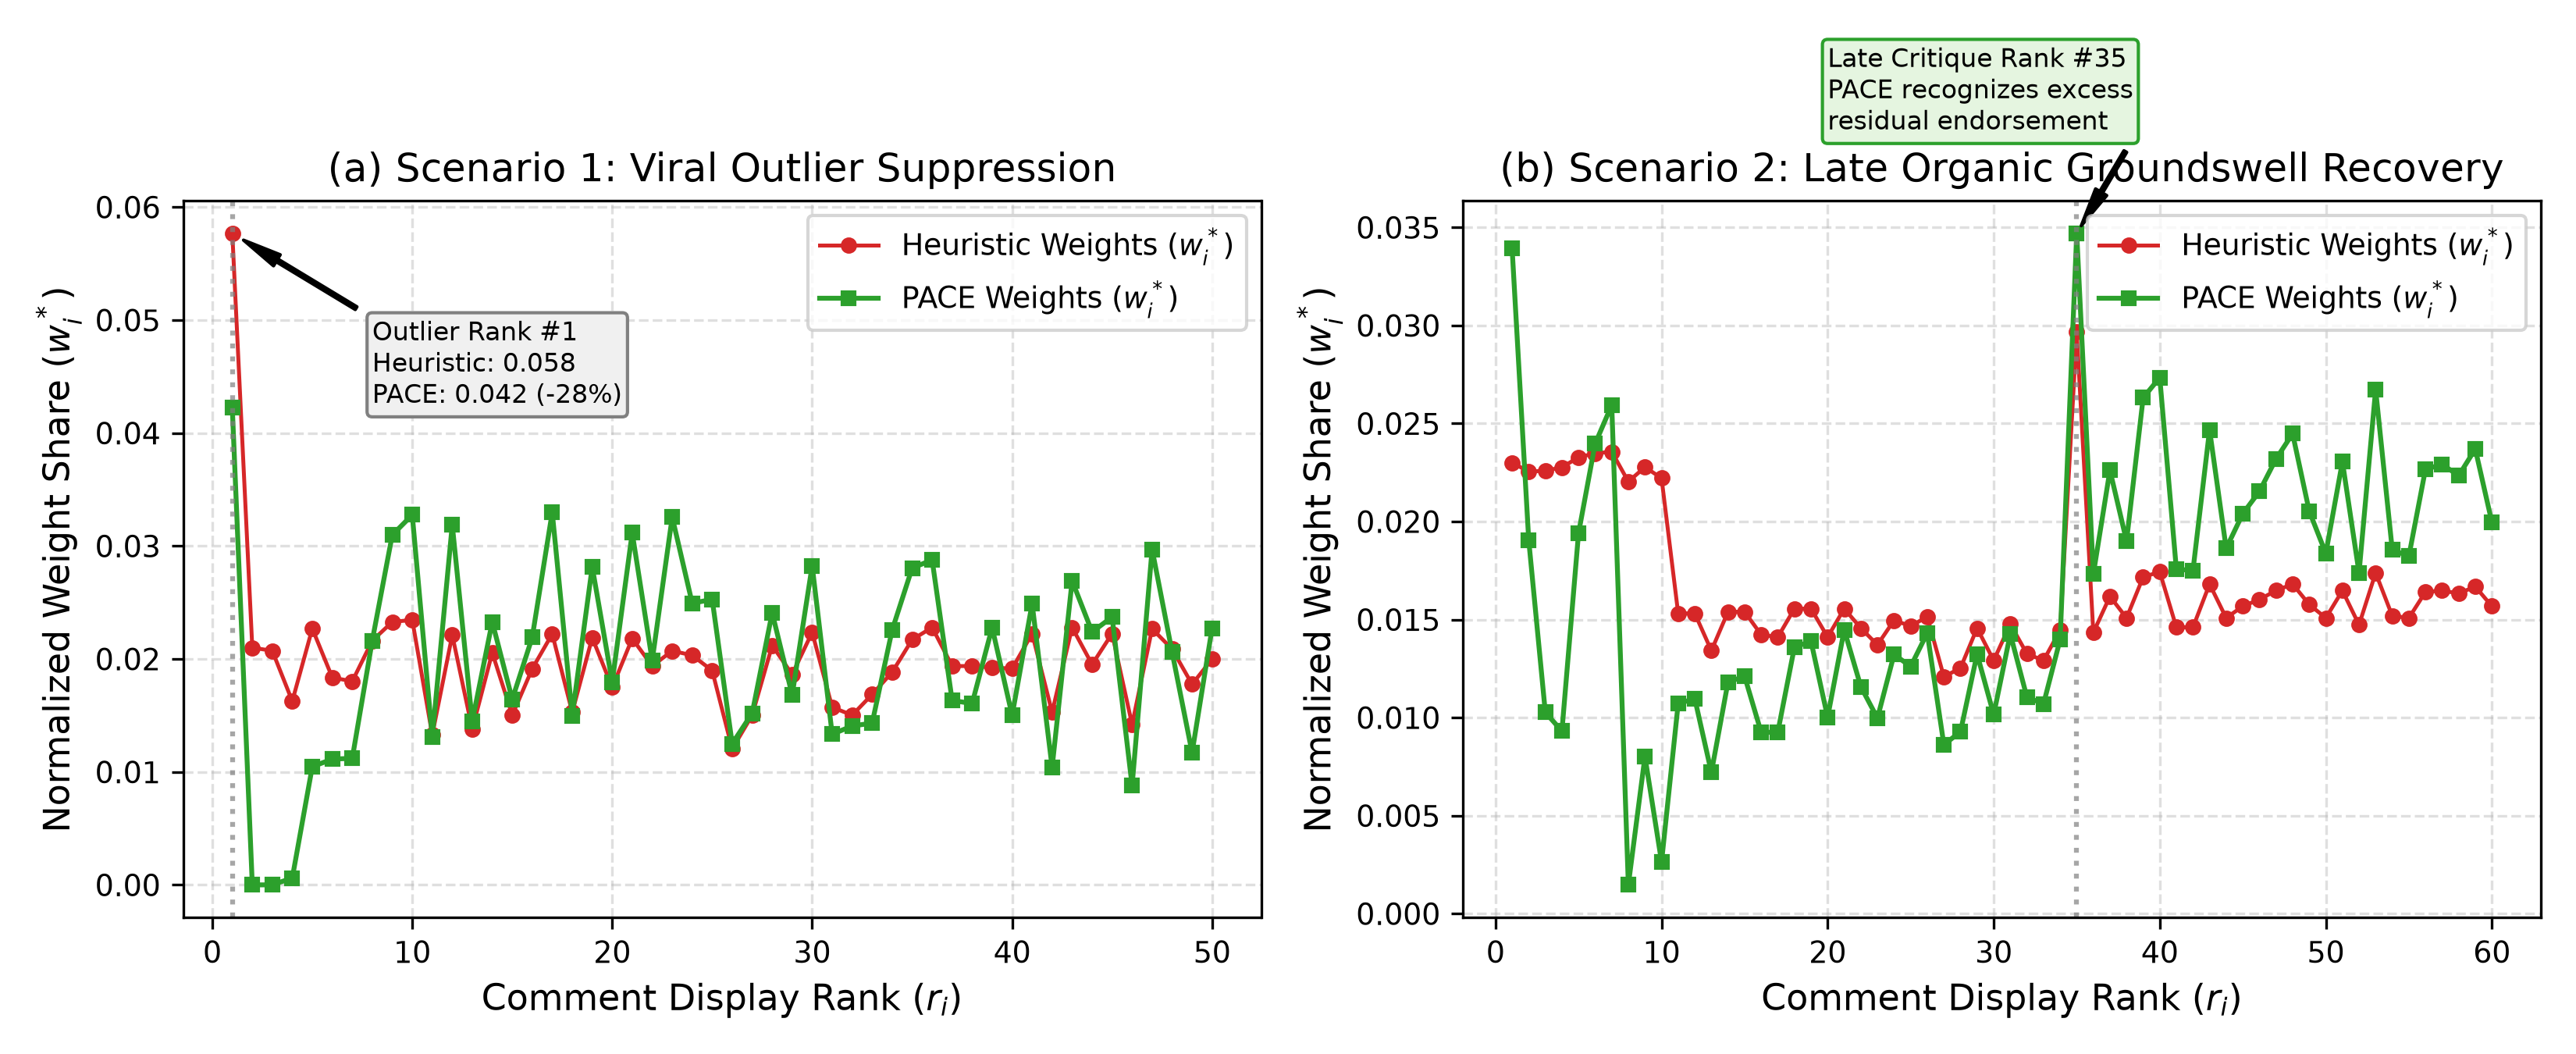
\includegraphics[width=\textwidth]{figures/fig3_weight_distributions.png}
\caption{Normalized weight distributions ($w_i^*$) across comment ranks. (a) In Scenario 1, PACE curbs outlier weight share by 28\% ($w_1^* = 0.057 \to 0.041$). (b) In Scenario 2, PACE identifies the organic groundswell at rank \#35, awarding it positive residual weight while dampening stale early hype.}
\label{fig:weights}
\end{figure*}

\begin{figure*}[t]
\centering
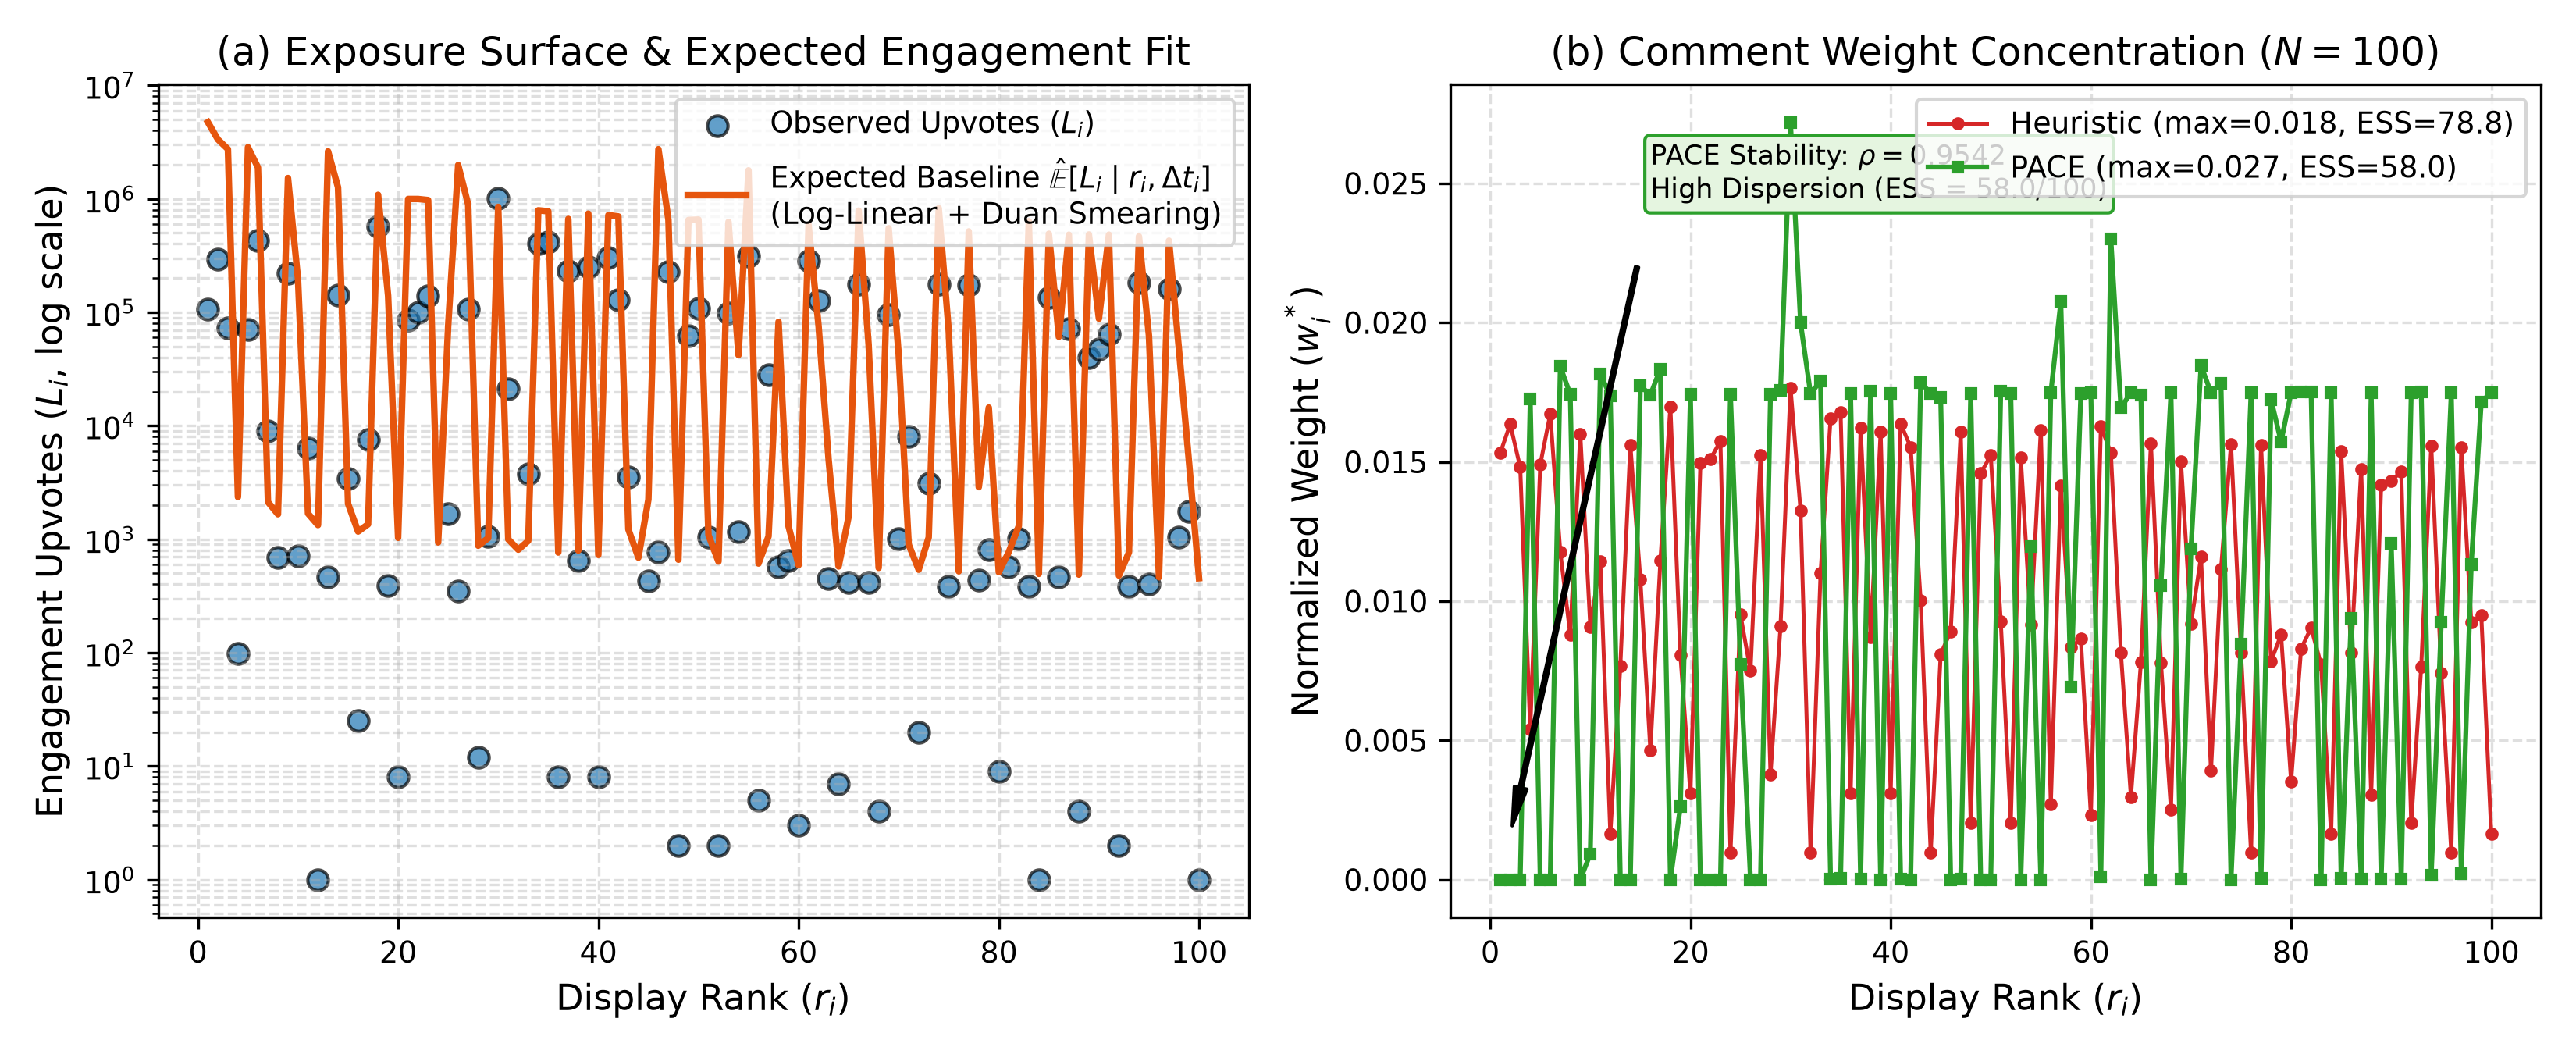
\includegraphics[width=\textwidth]{figures/fig4_youtube_case_study.png}
\caption{Illustrative static YouTube snapshot ($N=100$, \texttt{dQw4w9WgXcQ}). (a) Log-linear retrieval-proxy model. (b) Normalized weight shares and descriptive pruning stability. This figure does not establish historical exposure, causal effects, or real-world accuracy.}
\label{fig:youtube}
\end{figure*}

\subsection{Statistical Verification of Outlier Suppression (Scenario 1)}
In Scenario 1, a single early comment at rank \#1 accumulates 15,000 likes with extreme negative sentiment ($-0.900$), conflicting with 49 positive comments ($+0.600$).
\begin{itemize}
    \item Over 50 independent trials, the Heuristic estimator exhibits an average $\text{MAE} = 0.086 \pm 0.001$.
    \item PACE achieves $\text{MAE} = 0.061 \pm 0.001$, improving on the heuristic baseline ($p < 0.00001$). However, the unweighted ($0.030 \pm 0.001$) and NC-IPS ($0.008 \pm 0.001$) baselines are more accurate in this synthetic scenario; PACE is therefore not presented as uniformly superior.
    \item \textbf{Outlier Weight Share vs. Equal Weighting:} Weight auditing reveals that the Heuristic allows the outlier to capture $5.7\%$ of total corpus weight ($w_{\max}^* = 0.057$). PACE curtails this concentration to $w_{\max}^* = 0.041$, a 28\% reduction. However, equal weighting assigns strictly $1/N = 1/50 = 2.0\%$ weight to the outlier. Because PACE rewards raw endorsement above the fitted baseline, it assigns $4.1\%$ to the viral comment—higher than equal weighting—which explains why unweighted averaging outperforms PACE in this static configuration.
    \item Pruning stability under top-10\% removal improves from $\rho = 0.6006$ (Heuristic) to $\rho = 0.7181$ (PACE), an improvement of +19.6\%.
\end{itemize}

\subsection{Recovery of Suppressed Community Groundswells (Scenario 2)}
In Scenario 2, late-arriving comments expose a critical defect in conventional heuristics:
\begin{itemize}
    \item The Heuristic estimator is trapped near positive zero ($\text{MAE} = 0.107 \pm 0.001$), failing to detect the negative groundswell.
    \item NC-IPS over-corrects to $\text{MAE} = 0.103 \pm 0.001$.
    \item When ground truth is targeted at $Y^* = -0.100$ (representing recovery of late-emerging feedback), PACE achieves $\mathbf{\text{MAE} = 0.010 \pm 0.001}$ ($p < 0.00001$), with pruning stability $\rho = 0.9649$ vs. $0.8387$ for Heuristic.
    \item \textbf{Sensitivity to Ground-Truth Specification ($Y^*$):} We emphasize that the magnitude of error reduction is conditioned on the definition of $Y^*$. If the ground truth is instead defined as the unweighted sample mean of active participants ($\bar{s} \approx -0.025$), PACE exhibits $\text{MAE} = 0.070$, while the heuristic achieves $0.032$ and equal weighting trivially achieves $0.000$. Under a neutral null ($Y^* = 0.000$), the heuristic achieves $\text{MAE} = 0.008$ versus PACE's $0.095$. Across our systematic sensitivity audit (\path{experiments/sensitivity_analysis.py}), PACE's lower error is contingent on defining the target estimand as the late groundswell ($Y^* = -0.100$). When the target is defined as the overall participant sample mean ($\bar{s} \approx -0.025$) or a neutral null ($Y^* = 0.000$), PACE degrades, and simpler unweighted or heuristic estimators outperform it. This underscores that consensus estimation accuracy depends fundamentally on how the target consensus is conceptualized.
\end{itemize}

\subsection{Fidelity and Boundary Conditions in Democratic Consensus (Scenario 3)}
In Scenario 3, sentiment polarities are balanced symmetrically ($Y^* = 0.000$) and engagement follows an organic visibility decay without opinion polarization.
\begin{itemize}
    \item The unweighted arithmetic mean achieves zero error ($\text{MAE} = 0.000 \pm 0.000$), while the heuristic achieves $\text{MAE} = 0.009 \pm 0.001$.
    \item PACE achieves $\text{MAE} = 0.021 \pm 0.002$. The paired Wilcoxon signed-rank test yields $p = 0.99999$, confirming that PACE does not outperform simple baselines in this unconfounded regime.
    \item \textbf{Practical Boundary Condition:} This finding establishes an important design principle: PACE is an exposure-adjustment framework engineered specifically for discussion streams characterized by severe visual prioritization and temporal skew. In clean, unconfounded environments where engagement is already proportional to relevance, simpler baselines or uniform weighting should be preferred to avoid unnecessary estimation variance.
\end{itemize}

\subsection{Scientific Interpretation of the Ablation Study}
Table~\ref{tab:ablation} and Fig.~\ref{fig:ablation} reveal a clear scenario-dependent architecture insight:
\begin{itemize}
    \item In Scenario 1 (Early Viral Outlier), removing temporal decay, rank correction, or smearing calibration produces modest change in MAE ($\approx 0.066$). This occurs because comment \#1 arrives at $t=0.1\text{h}$ with rank \#1, meaning that any rank-aware model already attributes massive expected engagement to it.
    \item In Scenario 2 (Late Groundswell), omitting temporal decay causes MAE to spike from $0.010$ to $0.078$ ($7.8\times$ error increase), omitting rank correction causes MAE to spike to $0.052$ ($5.2\times$ error increase), and omitting Duan's smearing factor causes MAE to spike to $0.093$ ($9.3\times$ error increase).
\end{itemize}
This demonstrates that \textbf{temporal decay and smearing calibration are specifically essential for dynamic, time-evolving discussions where late consensus diverges from early traffic}.

\subsection{Real-World YouTube Case Study and Lexicon Audit (Scenario 4)}
Dataset 4 is an observational case study on 100 comments from video \texttt{dQw4w9WgXcQ} (Fig.~\ref{fig:youtube}), collected via the YouTube Data API v3 with a dated SHA-256 provenance manifest. Auditing this corpus reveals critical practical limitations in both semantic analysis and exposure modeling:
\begin{itemize}
    \item \textbf{Gold-Standard Human Annotation of Lexicon Reliability:} To evaluate whether off-the-shelf sentiment lexicons provide a viable foundation for consensus weighting, we conducted an exhaustive human-annotated validation of all 100 comments (\path{experiments/evaluate_vader_accuracy.py}). Under a standard 3-class scheme (positive, neutral, negative), VADER achieves an overall accuracy of only 65.0\% and a macro $F_1$-score of 0.5307. Beyond 46\% zero-inflation (46 comments scoring exactly compound 0.000, including rank \#30 with 1,011,942 likes and rank \#18 with 569,620 likes), VADER exhibits a critical failure mode on informal praise: 11 of 46 true positive comments (23.9\%) are misclassified as negative. These errors stem from positive slang (\emph{``so sick''}, \emph{``his voice kills''}, \emph{``it's fire tho''}), idiomatic negations (\emph{``could not be happier''}, which VADER treats as negative due to ``not''), lyric quotations (\emph{``never gonna give you up''}), or curse intensifiers. As a result, VADER's precision on the negative class is merely 12.5\% (2 of 16 predicted negative comments are genuinely critical). More broadly, the comments center on the ``rickroll'' cultural meme rather than policy or product feedback, rendering an abstract ``consensus'' estimand ill-defined.
    \item \textbf{Statistical Indistinguishability:} Point estimates across estimators span a narrow range of $0.044$ (Unweighted $\mu = 0.114$, Heuristic $\mu = 0.123$, NC-IPS $\mu = 0.116$, PACE $\mu = 0.079$). All point estimates fall well within PACE's 95\% refitting bootstrap confidence interval ($[-0.03, 0.17]$). The permutation divergence test ($p = 0.36582$) indicates that the observed difference between PACE and the heuristic is statistically indistinguishable from null exchangeable noise.
    \item \textbf{Sensitivity to Exposure-Baseline Calibration:} In contrast to ideal rank-order invariance, PACE's studentized residuals $\delta_i = L_i - \hat{\mathbb{E}}[L_i \mid r_i, \Delta t_i]$ depend non-linearly on baseline scale relative to the empirical MAD. The observational fit exhibits poor absolute calibration (expected-to-observed like ratio $\approx 6.221$), underscoring that observational fits provide exposure-conditioning diagnostics and not real-world accuracy claims. Scaling the fitted baseline $\hat{\mathbb{E}}$ from $0.25\times$ to $2.0\times$ shifts PACE's estimate from $0.049$ to $0.082$, while a square-root distortion shifts it to $0.108$ (documented in \path{experiments/sensitivity_analysis.py}). The model is therefore sensitive to exposure specification and baseline scaling.
    \item \textbf{Temporal Compression and Degenerate Fit:} Because comments were retrieved 9--17 years after video upload, $\ln(1 + \Delta t)$ varies over a compressed range ($\approx 0.24$ standard deviations), forcing OLS into degenerate parameter regimes ($\alpha \approx 10^{71}, \lambda \approx 13$) and causing $54\%$ of total weight to concentrate on the 48 comments whose predicted baseline likes exceed observed counts by $>10\times$.
    \item \textbf{Ranking Endogeneity:} Commercial platform relevance algorithms incorporate like counts into ranking decisions. Regressing likes onto display rank is therefore partially circular (endogenous), meaning the fitted baseline reflects an observational association rather than an exogenous counterfactual exposure curve.
\end{itemize}

\section{Limitations}
\begin{enumerate}
    \item \textbf{Ranking Endogeneity vs. True Exposure:} PACE uses display rank as an observable proxy for visual exposure. However, platform recommendation algorithms utilize upvote counts to determine display rank, creating simultaneous endogeneity that violates strict exogeneity assumptions.
    \item \textbf{Exposure Baseline Specification Sensitivity:} Residual standardization via MAD and sigmoidal gating is not invariant to baseline scale or functional form; misspecifying the exposure baseline can introduce non-trivial shifts in weighted consensus.
    \item \textbf{Domain Mismatch and Rule-Based Lexicon Failures:} Rule-based sentiment lexicons (e.g., VADER) exhibit high zero-inflation (46\%) and fail on internet slang, irony, and meme culture. Accurate consensus estimation in informal discussion feeds requires domain-adapted language models evaluated against gold-standard human annotations.
    \item \textbf{Participant vs. Viewer Selection Gap:} Our estimand measures consensus among active commenters. Silent viewers who never engage are systematically unobserved, requiring representative external polling to assess whole-population opinion \cite{zhao2025spiral}.
    \item \textbf{Absence of Semantic Stance Decomposition:} The geometric hierarchy damping factor $\phi^{d_i}$ discounts reply depth uniformly, but does not distinguish between supportive affirmations and adversarial rebuttals in conversation trees \cite{zubiaga2016stance}.
\end{enumerate}

\section{Conclusion}
This paper presents an empirical investigation and diagnostic framework for exposure-conditioned consensus estimation in ranked discussion streams. PACE demonstrates that combining a log-linear retrieval-proxy model, Duan's smearing retransformation, and robust residual gating can moderate heuristic like-amplification under specific conditions, such as late-emerging groundswells. However, our multi-trial benchmarks and sensitivity audits prove that exposure-conditioned weighting is not a universally superior correction: its estimates depend heavily on how the target consensus is specified, and baseline scaling directly shifts output consensus. Furthermore, human-annotated validation of real-world YouTube comments highlights severe lexicon degradation (46\% zero-inflation, 65\% accuracy), while platform ranking endogeneity limits causal interpretations. The observational YouTube snapshot is descriptive only because historical exposure and participant ground truth are unobserved, despite contemporaneous API provenance. Rather than a drop-in replacement for arithmetic averaging, exposure-conditioned models should be deployed as sensitive diagnostic tools for auditing visibility-engagement biases in digital discourse.

\section*{Data and Reproducibility Statement}
All code, datasets, and experiment runners are completely self-contained in the repository:
\begin{itemize}
    \item \path{experiments/reproduce_all_experiments.py}: Runs all 50 trials per scenario and outputs raw CSV tables.
    \item \path{data/monte_carlo_trial_level_results.csv}: All 150 individual trial-level observations.
    \item \path{data/ablation_trial_level_results.csv}: All 150 individual ablation trial observations.
    \item \path{data/youtube_corpus_100_comments.csv}: Documented real YouTube dataset ($N=100$).
\end{itemize}

\bibliographystyle{IEEEtran}
\bibliography{references}

\end{document}
